\newpage
\section{ Árboles de Decisión y Bosques Aleatorios}
\noindent Sea un vector aleatorio $\textbf{x}$ con $p$ los datos de entrada, e $Y$ la variable respuesta. Supóngase también que se toman $N$ observaciones obteniéndose parejas $(\textbf{x}_i,y_i)$. De esta manera, tenemos que las $\textbf{x}_i\in \mathbb{R}^p$.

\noindent Los métodos de árboles son un método divisivo, ya que tras aplicarlos, se obtiene una partición del espacio de observaciones $\mathbb{R}^p$ y luego en cada región del espacio se ajusta un modelo más simple, incluso una constante.

\noindent La ventaja de este tipo de métodos es que son fácilmente interpretables, ya que pueden ser representados mediante un diagrama de tipo árbol. De esta manera, pueden ser utilizados según \textit{Brown et.al}.\cite{Brown 2004} y \emph{Song Y.Y y Ying, L} \cite{Song 2015} describen los principales objetivos de los árboles de decisión, entre los que se encuentran la selección y evaluación de la importancia de las variables, además de que puede tener fines predictivos o incluso de manejo de los datos, valores perdidos etc...

\noindent Otra ventaja de este tipo de métodos es que permite trabajar con conjuntos de datos en los que se estudian más variables en comparación de las observaciones, es decir, $p > N$. Por ejemplo, el ejemplo que desarrollan \textit{Díaz-Uriarte y De Andrés} \cite{Diaz 2006}, en el que trabajan con un microarray genético. 

\noindent Otro de los problemas que surgen del propio planteamiento del modelo en sí es que el algoritmo para obtener las divisiones están diseñados para sobreajustarse a los datos por tanto, surgen métodos como la ``poda''. Se desarrollará más adelante, pero el idea es poder modelizar toda la variación del conjunto de entrenamiento. 

\subsection*{Notación}

\begin{defi}
Se llama \emph{separación, partición o división} de índice $(j,s)$ \cite{Hastie 2001} a la separación que particiona el espacio inicial dado en las siguientes regiones $R_1,R_2$:
\begin{equation}
R_1=\lbrace \mathbf{x}_i \in \mathbb{R}^p/ x_{ij}>s\rbrace \quad R_2=\lbrace \mathbf{x}_i \in \mathbb{R}^p/ x_{ij}\leq s\rbrace
\end{equation}

\noindent Hay que tener en cuenta que esto sería el caso en el que la variable a separar $X_j$ sea continua, en caso, contrario, se puede definir la partición $(j,s)$ de la siguiente manera: 

\end{defi}

\begin{defi}
Se llama nodo de un árbol de decisión a cada una de las regiones resultantes tras aplicar una separación.
\end{defi}

\begin{defi}
Se llama nodo terminal de un árbol de decisión a las regiones finales en las que se ha particionado el espacio de observaciones. 
\end{defi}

\begin{defi}
Llamaremos tamaño del árbol $T$, $|T|$ al número de nodos terminales. 
\end{defi}

\begin{defi}
Se llama profundidad del árbol al número máximo que de divisiones que hay que hacer para llegar a un nodo terminal. \emph{En el caso del diagrama que se incluye después se dan 3 divisiones del espacio tanto para llegar a $R_4, R_5$}
\end{defi}

\noindent Las  anteriores imágenes procedentes de \textit{Hastie et. al.}\cite{Hastie 2001} muestran el diagrama resultante tras dividir el espacio de observaciones mediante un árbol. 

\begin{figure}[h]
 \centering
  \subfloat[División de $\mathbb{R}^p$]{
   \label{f:división}
    \includegraphics[width=0.4\textwidth]{Documentos Extra/Imagenes/Regiones árboles.png}}
  \subfloat[Diagrama resultante]{
   \label{f:diagrama arbol}
    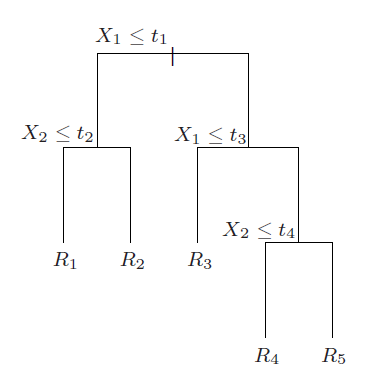
\includegraphics[width=0.4\textwidth]{Documentos Extra/Imagenes/Diagrama de arbol.png}}
 \caption{Representación de la división de $\mathbb{R}^p$ y el diagrama de árbol resultante}
 \label{f:MARC1}
\end{figure}

\noindent Como se puede ver, cada uno de los nodos terminales representan cada una de las regiones en las que se ha separado el espacio de observaciones. 

\noindent Dependiendo del tipo de variable respuesta, tendremos un tipo de árbol u otro, por ejemplo, cuando la variable sea continua se denominará \emph{Árbol de regresión} y en el caso de variables discretas \emph{Árbol de clasificación}. En nuestro caso, todos los tipos de algoritmos que se detallarán las variables de entrada pueden ser tanto discretas como continuas.  Habitualmente, se detallará el caso en el que las variables de entrada son continuas.

\subsection*{Sesgo y varianza de un modelo}

\noindent Un aspecto en el que no se ha indagado en el trabajo por ahora es en la capacidad predictiva de los modelos. Es decir, a la capacidad de obtener dadas nuevas observaciones $\mathbf{x}_0$ de las variables predictoras, hallar el valor que tendría la variable respuesta $Y$. 

\noindent Supóngase variable respuesta sigue un modelo del tipo $Y=f(\mathbf{x})+\varepsilon$, en el que la variable aleatoria $\varepsilon\sim N(0,\sigma^2)$ y la variable respuesta $Y\sim N(f(\mathbf{x}),\sigma^2)$ conociendo el vector de variables predictoras. Si la $f(\mathbf{x})$ fuera una función lineal y la variable respuesta $Y$ fuera continua, se estaría ante un modelo de regresión lineal por ejemplo. 

\noindent Consideremos que se toma una muestra con  $N$ observaciones, obteniéndose una matriz de datos $\mathbf{X}$, la matriz de respuesta $\mathbf{Y}$ y que se ajusta el modelo y sus parámetros conocidas conociendo estas $N$ observaciones. Entonces, para una nueva observación de las variables predictoras $\mathbf{x}_0$, se puede definir el siguiente concepto \cite{Hastie 2001, Lawless 2010}:

\begin{defi}
Se llama \emph{error de predicción esperado} de la observación $\mathbf{x}_0$ a la siguiente expresión:
\begin{equation}
EPE(\mathbf{x}_0)=\mathbb{E}((Y-\hat{Y})^2|\mathbf{x}=\mathbf{x}_0)=\mathbb{E}((Y-\hat{f}(\mathbf{x}_0))^2)
\end{equation}
\end{defi}
\noindent De esta manera, se tiene una forma de medir el rendimiento predictivo de un modelo. Es por ello, también que en aplicaciones de aprendizaje automático en las que se busca hacer predicciones lo más precisas posibles, se divide el conjunto de datos en el conjunto de entrenamiento y de validación ya que una vez ajustado el modelo, se evalúa su capacidad predictiva mediante un estimador del error de predicción esperado con una muestra aparte de los datos de entrenamiento o ajuste.

\noindent Este error de predicción se puede descomponer de manera sencilla 
\begin{propo}
El error de predicción esperado se puede dividir en un termino irreducible, el sesgo del modelo y la varianza \cite{Hastie 2001}:
\begin{equation}
EPE(\mathbf{x}_0)=\sigma_{\varepsilon}^2+Sesgo(\hat{f}(\mathbf{x}_0))^2+Var(\hat{f}(\mathbf{x}_0))
\end{equation}
\noindent Donde el $Sesgo(\hat{f}(\mathbf{x}_0))=\mathbb{E}(f(\mathbf{x}_0)-\hat{f}(\mathbf{x}_0))$.
\begin{proof}
\begin{align*}
\mathbb{E}((Y-\hat{f}(\mathbf{x}_0))^2)&=\mathbb{E}((Y-f(\mathbf{x}_0)+f(\mathbf{x}_0)-\hat{f}(\mathbf{x}_0))^2)=\\
&=\mathbb{E}(\varepsilon^2)-2\mathbb{E}(\varepsilon\cdot(f(\mathbf{x}_0)-\hat{f}(\mathbf{x})_0))+\mathbb{E}((f(\mathbf{x}_0)-\hat{f}(\mathbf{x}_0))^2)\\
&=\sigma^2+\mathbb{E}((f(\mathbf{x}_0)-\hat{f}(\mathbf{x}_0))^2)
\intertext{El segundo término es el error cuadrático medio de un estimador, luego se obtiene que:}
\mathbb{E}((Y&-\hat{f}(\mathbf{x}_0))^2)=\sigma^2+Sesgo(\hat{f}(\mathbf{x}_0))^2+Var(\hat{f}(\mathbf{x}_0))
\end{align*}
\end{proof}
\end{propo}

\noindent Estos dos parámetros están íntimamente relacionados con la complejidad del modelo, ya que cuanto más complejo sea el modelo, el sesgo se reduce de manera importante. Esto es debido a que los puntos del conjunto de entrenamiento están bastante cerca de las funciones aproximadas, en cambio la varianza se dispara, lo que implica que a la hora de hacer predicciones estas no sean lo mejor posible \cite{Neural Designer}. 

\noindent Para el caso en el que tengamos un modelo lineal que \emph{Hastie et. al.} \cite {Hastie 2001} desarrolla, se ve que la varianza del error esperado medio en observaciones del conjunto de entrenamiento depende de $\frac{p}{N}$, y el sesgo de $\frac{1}{N}$. Por tanto, a mayor numero de observaciones y menor de variables predictoras mejor. Esto se puede observar en el siguiente gráfico que incluyen \emph{Hastie et.al.} \cite{Hastie 2001} de manera que se puede ver a mismo número de observaciones que pasa si aumentamos las variables observadas. La línea roja representa lo que ocurre con el error de predicción en observaciones fuera del conjunto de ajuste y la azul representa dentro del conjunto de ajuste. 

\noindent Esta parte se va utilizar, tanto en los árboles como en los random forests, ya que son métodos que buscan con un conjunto relativamente pequeño de observaciones en relación con el numero de variables observadas obtener un modelo que no tenga un sobre ajuste excesivo. De hecho, para hacer crecer un árbol, se busca hacerlo crecer hasta un punto de sobre ajuste y luego se irá ``podando" de la manera que se definirá más tarde para evitar dicho sobre ajuste introduciendo algo de sesgo. 
%\begin{figure}[h]
%\centering
%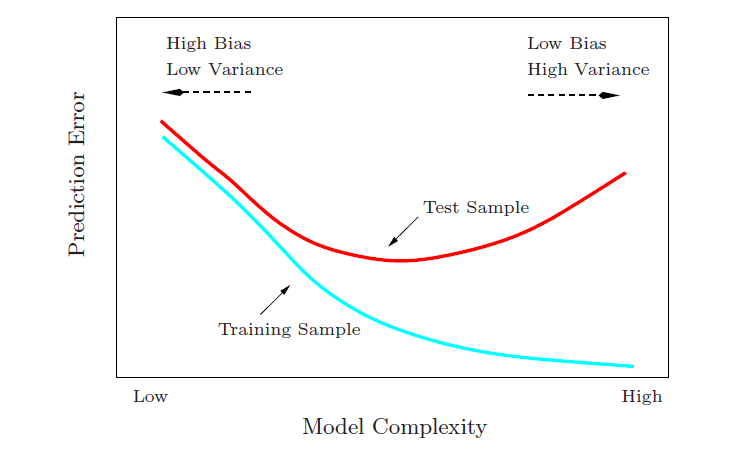
\includegraphics[scale=0.3]{Documentos Extra/Imagenes/Bias-Variance-Tradeoff.png}
%\end{figure}
 
\newpage
\subsection{Árboles de Regresión}

\noindent Veamos ahora el proceso por el cual se hace ``crecer'' un árbol, en particular un árbol de regresión en el que se dispone de un vector aleatorio $\mathbf{x}$ de $p$ variables aleatorias  predictoras, y una variable respuesta continua $Y$. 

\noindent Supongamos prefijado el número máximo de particiones $M$, por tanto el objetivo del árbol de decisión es particionar el espacio de observaciones en las regiones $R_m, m=1,\ldots, M$ , teniendo en cuenta esto, $R_m$ tiene asociada su \emph{función característica} que denotaremos por $\mathbf{1}_m$. 

\noindent \emph{Observación: } El número de regiones obtenidas al final es el tamaño del árbol, $|T|=R_m$ 

\noindent En el caso de que se tomen $N$ observaciones como se ha hecho en anteriores secciones, podemos definir el estimador $\hat{f}(\mathbf{x})$ de la siguiente manera: 

\begin{equation}
\hat{f}(\mathbf{x})=\sum_{m=1}^M \hat{f}_m(\mathbf{x})\cdot \mathbf{1}_m(\mathbf{x})
\end{equation}

\noindent Es decir, en cada región $R_m$, se hace una regresión con los datos que se den en esa región. Lo más común es que en cada región se intente tomar la aproximación lo más sencilla posible, es decir, una constante \cite{Hastie 2001,Biau 2016}.

\noindent  Si se aplica el método de los mínimos cuadrados, con la restricción requerida, se pueden definir las constantes $\hat{c}_m$ de la siguiente manera:
\begin{equation}
\hat{c}_m=\dfrac{1}{N_m}\sum_{i/\mathbf{x}_i\in R_m} y_i
\end{equation}
\noindent Es decir, es la media de las respuestas de las observaciones que entran en la región y esto provoca que $\hat{f}(\mathbf{x})=\sum_{m=1}^M \hat{c}_m \cdot \mathbf{1}_m(\mathbf{x})$. 

\noindent Una vez se conoce como se va a dar la estimación final hay que saber cómo llegar a la mejor partición. A este proceso de elegir las particiones y elegir dichas particiones $(j,s)$. 

\noindent En regresión, hay que elegir $j$ y $s$ de tal manera que las regiones resultantes $R_{m_1},R_{m_2}$ son aquellas en las que se minimiza la siguiente expresión:
\begin{equation}
\sum_{i/\mathbf{x}_i\in R_{m_1} } (y_i-\hat{c}_{m_1})^2+\sum_{i/\mathbf{x}_i\in R_{m_2} } (y_i-\hat{c}_{m_2})^2
\end{equation}

\noindent Es decir, el objetivo es encontrar las separaciones que minimicen la suma de los errores cuadráticos. Podemos definir el error cuadrático medio de cada región de la siguiente manera \cite{Hastie 2001}.

\begin{defi}
Se llama error cuadrático medio de una región $R_m$ a $Q_m(T)=\frac{1}{N_m}\sum_{i/\mathbf{x}_i\in R_m}(y_i-\hat{c}_m)^2$.
\end{defi}

\noindent Por tanto, podemos definir una función de coste general 
\begin{equation}
Q(T)=\sum_{m=1}^M\frac{1}{N_m}\sum_{i/\mathbf{x}_i\in R_m} (y_i-\hat{c}_m)^2
\end{equation}

\noindent \emph{Divakaran, S. }\cite{Divakaran 2022},  detalla que el encontrar las mejores particiones que minimicen esta función de coste de un árbol de regresión es un problema altamente complejo a nivel computacional. Es por ello, que \emph{Breiman L.}\cite{Breiman 1984} especifica un algoritmo el cual utilizando mecanismos de validación cruzada, compara distintos modelos para crear un algoritmo voraz heurístico para afrontar el problema descrito. 

\noindent Para empezar hay que definir lo que significa la poda de un árbol. 
\begin{defi}
Se llama \emph{poda} al proceso en el que dado un árbol inicial de tamaño $T_0$ se revierten ciertas particiones terminales que no aportan en la relación coste-complejidad, es decir, aumentan demasiado la complejidad (\emph{Aumentando la varianza}), sin reducir el coste (\emph{Sesgo}).
\end{defi}

\noindent \emph{Divakaran, S. }\cite{Divakaran 2022}, propone añadir un término al coste del árbol. 
\begin{equation}
Q_{\alpha}(T)=\sum_{m=1}^M\frac{1}{N_m}\sum_{i/\mathbf{x}_i\in R_m} (y_i-\hat{c}_m)^2+\alpha|T |
\end{equation}



\subsection{Árboles de Clasificación}

\noindent Sea ahora el caso en el que las variables predictoras son como antes, dadas por un vector aleatorio $\mathbf{x}$ de longitud $p$ , discretas o continuas de manera indiscretas, pero en el que la variable respuesta es una variable aleatoria con $L$ posibles valores.

\noindent Tómense ahora $N$ observaciones simultáneas del vector $\mathbf{x}$ y la variable respuesta $Y$ para el cual se ha hecho crecer un árbol $T$ de tamaño $M$, entonces, podemos denotar de la siguiente manera \cite{Divakaran 2022, Brown 2004}
\begin{equation}
\hat{p}_{lm}=\text{Proporción de observaciones en las que $y_i=l$, en la región $R_m$.}
\end{equation}

\noindent Teniendo en cuenta esto, se pueden definir los siguientes conceptos.
\begin{defi}
Se dice que un nodo correspondiente a la región $R_m$ es puro, si $\exists l_0/ p_{l_0 m}=1$ y $\hat{p}_{lm}=0 \quad \forall l\neq l_0$ \cite{Divakaran 2022, Hastie 2001, James 2013, Brown 2004}. 
\end{defi}

\begin{defi}
Se define la \emph{impureza de un nodo}, correspondiente a la región $R_m$ como \cite{Brown 2004}:
\begin{equation}
1-\max_{l\in L} \hat{p}_{lm}
\end{equation}
\noindent Es decir, si se hablara de coste, estamos asumiendo que en esa región $R_m$, la $l$ tal que $\hat{p}_{lm}$ es máxima es la correcta. Entonces, la impureza se puede interpretar como la ``probabilidad" de error. 
\end{defi}
\noindent Otra forma de medir la impureza son el índice Gini y la entropía. \emph{Hastie et. al.} y \emph{Divakaran, S.} \cite{Hastie 2001, Divakaran 2022}, definen el índice Gini de la siguiente manera:
\begin{defi}
Se llama \emph{índice Gini} a la siguiente expresión \cite{Hastie 2001, James 2013}:
\begin{equation}
G=\sum_{}
\end{equation}
\end{defi}

\subsection{Bosques Aleatorios}

\noindent Los bosques aleatorios y otros métodos de juntar árboles de decisión son maneras de solventar ciertos problemas que tienen los árboles de decisión individuales como puede ser la precisión o la dependencia del conjunto de datos, ya que una pequeña variación en estos puede provocar grandes cambios. 


\noindent Durante esta sección no se detallarán los métodos de construcción de cada árbol individual ya que se han descrito anteriormente y se hará referencia a ellos como árboles simplemente. 

\noindent Estos métodos se basan en el  Bagging y el Bootstrap, ambos métodos se pueden utilizar cuando la cantidad de datos es pequeña o cuando el modelo sufre de \textit{sobreajuste}. 

\noindent El proceso de Bagging tiene como base el hecho de que si se tienen $n$ observaciones independientes de una población con varianza $\sigma^2$ entonces la media de dichas observaciones tendrá varianza $\frac{\sigma^2}{n}$, es decir, tomar la media de distintas observaciones provoca una disminución en la varianza. 


\noindent De esta manera, partiendo de un conjunto inicial de datos, se toman muestras aleatorias de los mismos y se entrenan distintos modelos para luego hacer la media entre todos los modelos. Es decir, se hace un muestreo aleatorio entre las $n$ observaciones obteniendo $B$ conjuntos de entrenamiento distintos y se estiman los predictores $\hat{f}_1(\textbf{x}),\ldots, \hat{f}_B(\textbf{x})$ y el modelo final es:
\begin{equation}
\hat{f}_{bag}(\textbf{x})=\dfrac{1}{B}\sum_{b=1}^B \hat{f}_b(\textbf{x})
\end{equation}

\noindent Esto se puede aplicar perfectamente al caso de la modelización mediante árboles de decisión aunque esta técnica puede ser útil para cualquier tipo de modelos. 

\noindent En este caso, estamos utilizando en cada división de los árboles todos los predictores, sin embargo, cuando una variable tiene demasiada importancia a la hora de predecir la variable de respuesta, la mayoría de divisiones en casi todos los árboles van a utilizar ese predictor, ya que va a provocar mejoras sustanciales en el $RSS$ o en el \textit{índice Gini} dependiendo del tipo de árbol. 

\noindent Para evitar dicho problema, en el algoritmo del bosque aleatorio se toma en cada división no el total de predictores, si no una muestra aleatoria de tamaño $m$ que habitualmente es $m=\sqrt{p}$ de esta manera, se puede tener modelos con mayor variedad. 

\noindent En \textit{Biau G. y Scornet E.}\cite{Biau 2016} se detalla el algoritmo para la creación de un bosque aleatorio. 
En este algoritmo se deben definir los siguientes parámetros:
\begin{itemize}
\item $\mathcal{M}$: Número de árboles que se incluirán en el bosque aleatorio. 
\item $\mathtt{m}_{\mathtt{try}}$, es el número de predictores que entre los cuales se pueden usar en cada división del espacio. 
\item $a_n$: Número de observaciones del conjunto de entrenamiento que se utilizarán para entrenar cada árbol. 
\end{itemize}

\noindent El algoritmo en sí es el siguiente: 
\hrule
\textbf{for } $j=1\ldots \mathcal{M} $ \textbf{do:}
\begin{itemize}
\item Se extrae de manera uniforme un subconjunto de tamaño $a_n$ del conjunto de observaciones de entrenamiento. 
\item Se extrae aleatoriamente un conjunto de predictores posibles $\mathcal{M}_{try}$ de tamaño $\mathtt{m}_{\mathtt{try}}$ y se construye el árbol, utilizando como posibles  predictores únicamente los que están en el conjunto $\mathcal{M}_{try}$
\end{itemize}
\hrule

\noindent Para hacer la predicción para una nueva observación $\textbf{x}_0$, hay que calcular la predicción para cada uno de los $\mathcal{M}$ árboles. Una vez calculadas en el caso de que la variable respuesta sea numérica se hace la media de todas las predicciones. Si por el contrario, $Y$ es una variable categórica, se toma como predicción aquella que haya salido con mayor frecuencia, lo que se llama predicción por \textit{voto de mayoría}.

\noindent En el artículo de \textit{Biau, G y Scornet, E.} \cite{Biau 2016} se detallan más en profudidad las distintas características de estos modelos. En particular, se detalla la necesidad de utilizar modelos simplificados para poder analizar las características de los bosques aleatorios. Estos pueden ser los bosques puramente aleatorios que hace particiones totalmente aleatorias sin tener un criterio de acuerdo a los datos y otras modificaciones.

\noindent En particular, \textit{Breiman L.} \cite{Breiman 2004}, utiliza los siguientes resultados empíricos para poder analizar la consistencia y el ratio de convergencia de los bosques aleatorios utilizando un modelo más simplificado de los mismos. 
\begin{itemize}
\item El muestreo aleatorio que se hace del conjunto de entrenamiento no tiene efecto en el ratio de error.
\item Si para conseguir una partición en la que únicamente en cada nodo haya una sola observación se utiliza la mediana de las variables aleatorias esto no tiene efecto en el ratio de error. 
\item Hacer divisiones sin tener en cuenta las clases que conocemos, sí aumenta el error.
\end{itemize}

\noindent De esta manera, establece un modelo simplificado en el las variables predictoras se pueden dividir en dos grupos, las variables fuertes $\mathcal{S}$ y las variables débiles $\mathcal{W}$. Las variables fuertes son las que tienen una influencia directa sobre las predicciones y las débiles se pueden interpretar como ruido.

\noindent Teniendo en cuenta lo anterior, las variables aleatorias fuertes se dividen en la mediana, mientras que si es débil se toma un valor aleatorio para la división.  

\noindent Como resultado de dichas modificaciones \textit{Breiman, L.} \cite{Breiman 2004} concluye que el ratio de convergencia es $\mathcal{O}\left(n^{\left(\frac{-0.75}{|\mathcal{S}|log 2+0.75}\right)}\right)$.\\
Por tanto, el ratio de error depende del número de variables fuertes. 

 